\documentclass[10pt]{article}
\usepackage[utf8]{inputenc}
\usepackage{empheq}
\usepackage[inline, shortlabels]{enumitem}
\usepackage{gensymb}
\usepackage{multicol}
\setlength{\parskip}{0.5cm plus4mm minus3mm}
\setlength{\parindent}{0pt}
\usepackage{amsmath}
\usepackage{upgreek}
\usepackage[nobreak=true]{mdframed}
\usepackage[shortlabels]{enumitem}
\usepackage[margin=0.8in]{geometry}
\usepackage{changepage}
\usepackage{amssymb}
\usepackage{tikz}
\usetikzlibrary{arrows}
\usepackage{cs170}
\usepackage{titlesec}
\usepackage{chngcntr}
\usepackage{graphicx}
\newcommand{\norm}[1]{\lvert #1 \rvert}
\newcommand{\Est}[1]{\hat{#1}}
\newcommand{\argmax}{\operatornamewithlimits{argmax}}
% \vspace{-5ex}
\begin{document}
\date{}
\title{\vspace{-5ex} 
\dunhd{EE16A: Designing Information Devices and Systems I Notes} \vspace{-5ex}}
\maketitle
\begin{multicols}{2}
\begin{enumerate}
    \item \textbf{Network Flows:} 
    \begin{align*}
        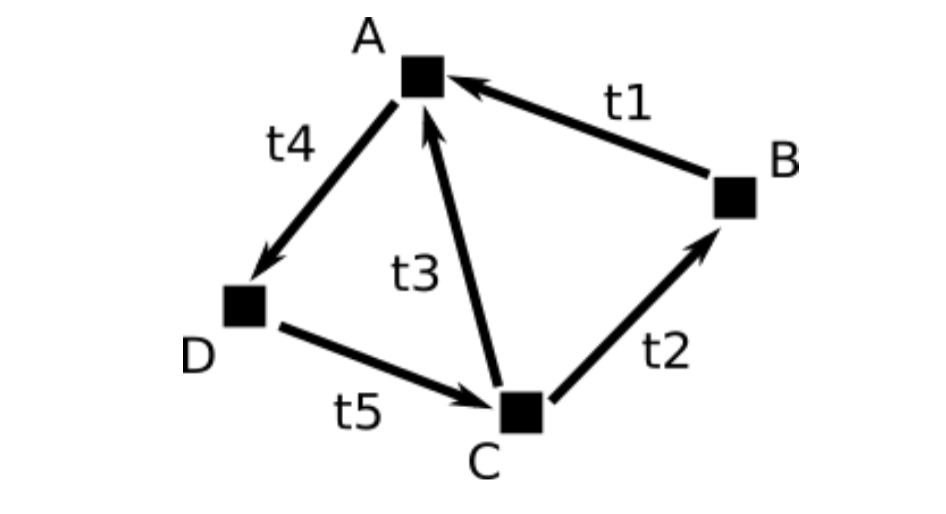
\includegraphics[scale=0.25]{Nodes.png}
     \end{align*}
    Construct the incidence matrix as follows:
    \begin{equation*}
        B=\begin{bmatrix} 
        1 & 0 & 1 & -1 & 0 \\
        -1 & 1 & 0 & 0 & 0 \\
        0 & -1 & -1 & 0 & 1 \\
        0 & 0 & 0 & 1 & -1
        \end{bmatrix}
        \begin{bmatrix} t_1 \\ t_2 \\ t_3 \\ t_4 \\ t_5 \end{bmatrix}=\vec{0}
    \end{equation*}
    The null space of $B$ is exactly the set of valid flow vectors. Construct a basis by solving $B\vec{t}=\vec{0}$.
    
    \item \textbf{Circuit analysis:}\\ First use \textbf{Kirchhoff's current law}: At any node (junction) in an electrical circuit, the sum of currents flowing into that node is equal to the sum of currents flowing out of that node. Write appropriate equations for EACH junction. Maintain consistency with choice of current direction. \\
    \textit{Example}:
    \begin{align*}
        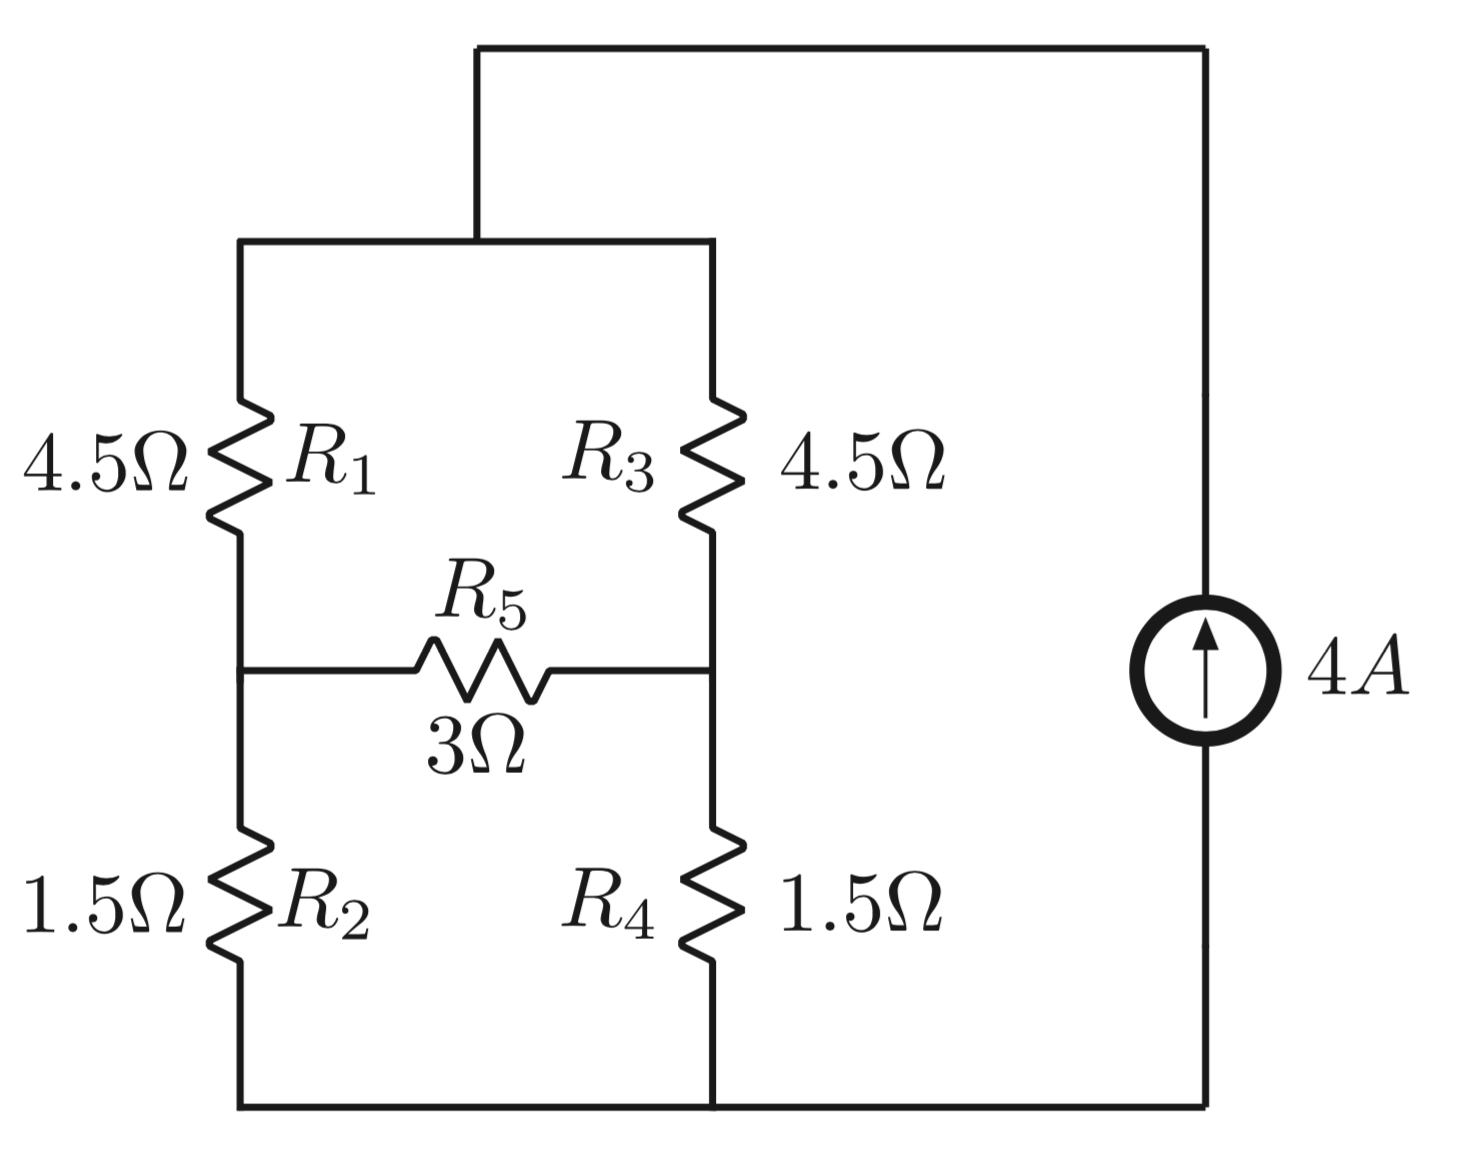
\includegraphics[scale=0.2]{Circuit2.png}
     \end{align*}
     Let $I_n$ denote the current across resistor $n$. From Kirchhoff's current Law, we see:
     \begin{align*}
         I_1 + I_3 &= 4 \\
         I_5 + I_2 &= I_1 \\
         I_5 + I_3 &= I_4 \\
         I_2 + I_4 &= 4 
     \end{align*}
     Then use \textbf{Kirchhoff's voltage law}: The sum of the products of the resistances and the currents in any closed path is equal to the total voltage available in that path.
     \begin{align*}
         4.5I_1 + 1.5I_2 = 4.5I_3 + 1.5I_4 \\
         4.5I_1 + 1.5I_4 = 4.5I_3 + 1.5I_2
     \end{align*}
     We put these equations into an augmented matrix and solve for the current across each resistor. To find the voltage across each resistor, we use Ohm's Law: $V=IR$.
    
    \item \textbf{Circuit Terms:}
    \begin{enumerate}
        \item \textbf{Voltage} is electric potential energy per unit charge, measured in joules per coulomb (Volts).
        \item \textbf{Current} is the flow of electric charge, measured in coulombs per second (Amps).
        \item \textbf{Resistance} is the impedance of current flow measured in Volts per Amps (Ohms $\Omega$). Thus $V=IR$. $R = \frac{\rho L}{A}$ where $L$ is length, $A$ is cross-sectional area, and $\rho$ is resistivity of material.
        \item \textbf{Power} is the rate of electrical energy usage, measured in Joules per second (Watts). $P=IV$.
        \item \textbf{Capacitance} represents how much charge can be stored for a given amount of voltage, measured in Coulombs per Volts (Farads). Thus $Q=CV$. $C= \varepsilon \frac{A}{d}$ where $A$ is surface area of plates, d is the separation and $\varepsilon$ is permitivity of the material between the plates.
        \item Note that according to passive sign convention, positive current goes into the positive terminal of a component.
    \end{enumerate}

    \item \textbf{Voltage Divider:} 
    \begin{align*}
        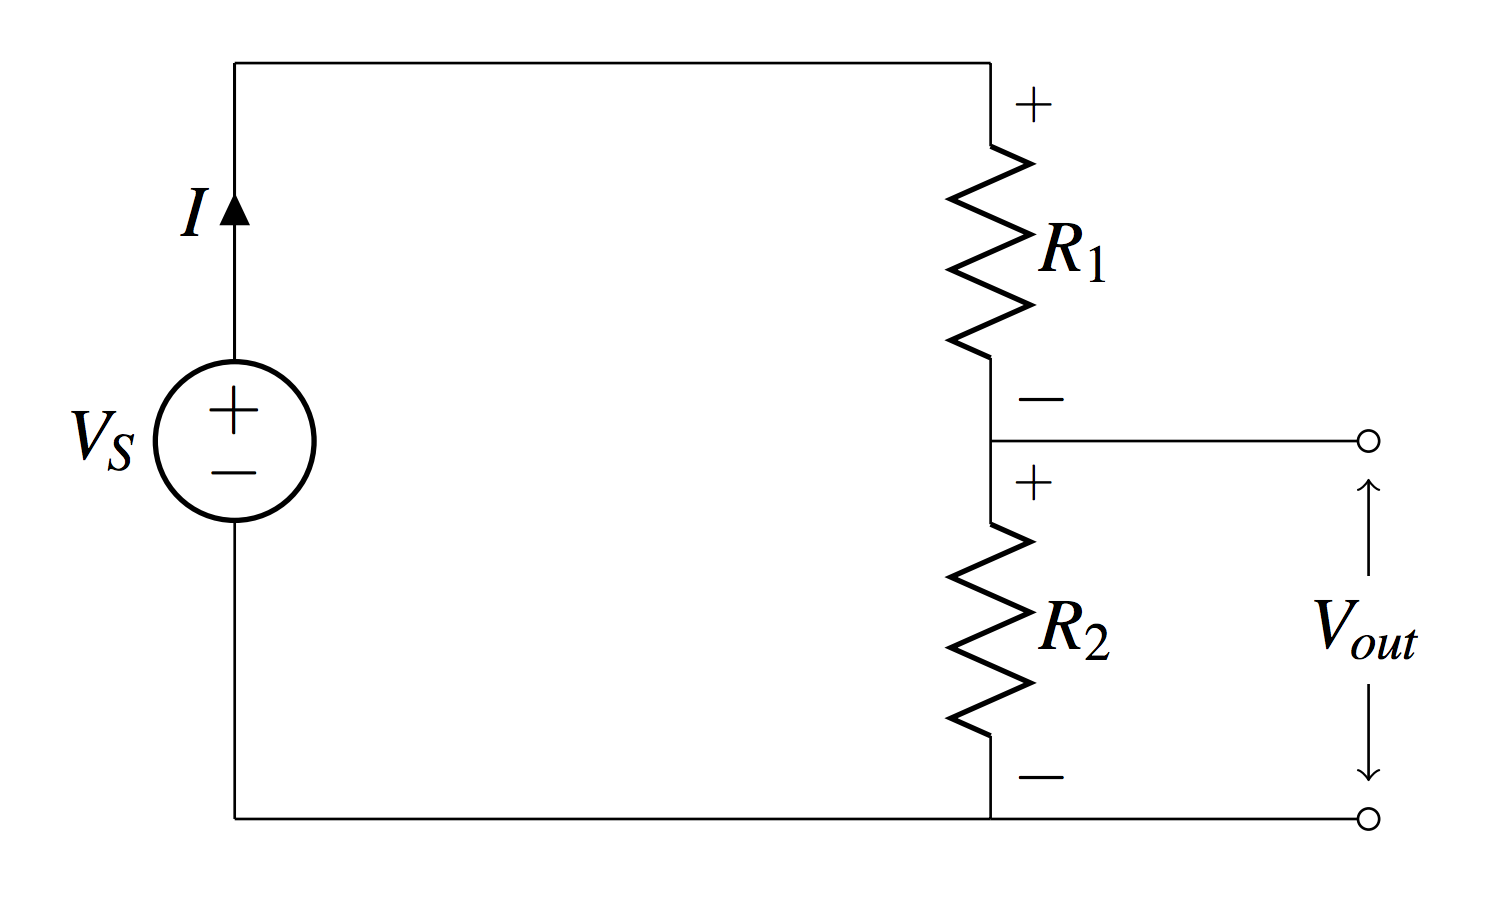
\includegraphics[scale=0.2]{voltage_divider.png}
     \end{align*}
     We can vary the output voltage by varying $R1$ and $R2$.
     \begin{equation*}
         V_{out} = \frac{R2}{R1+R2}V_S
     \end{equation*}
    
    \item \textbf{2D Resistive Touchscreen:} To measure vertical touch position: 
    \begin{align*}
        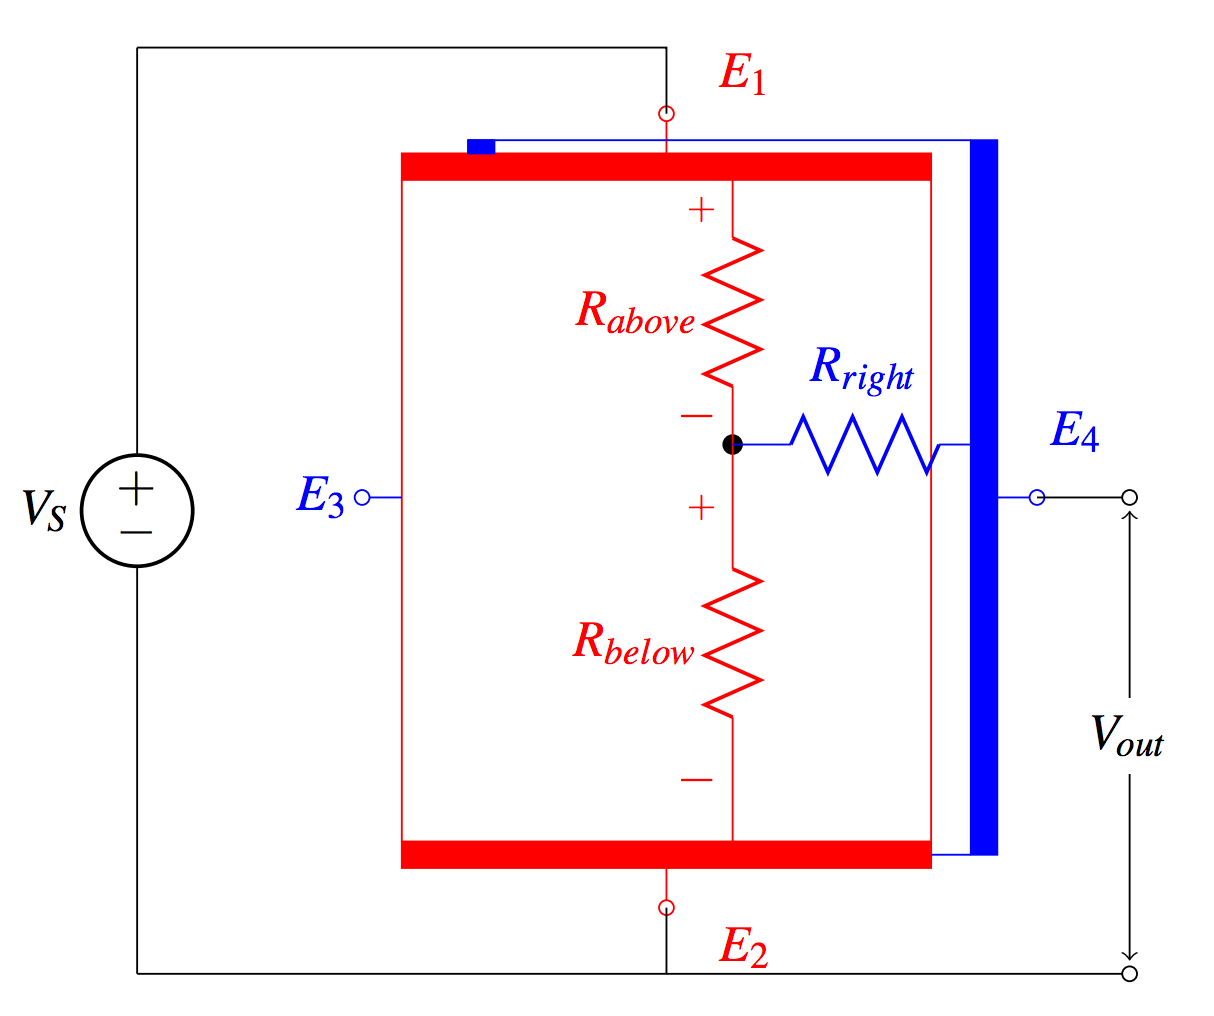
\includegraphics[scale=0.3]{vpos.png}
     \end{align*}
     Which simplifies to a simple voltage divider:
    \begin{align*}
        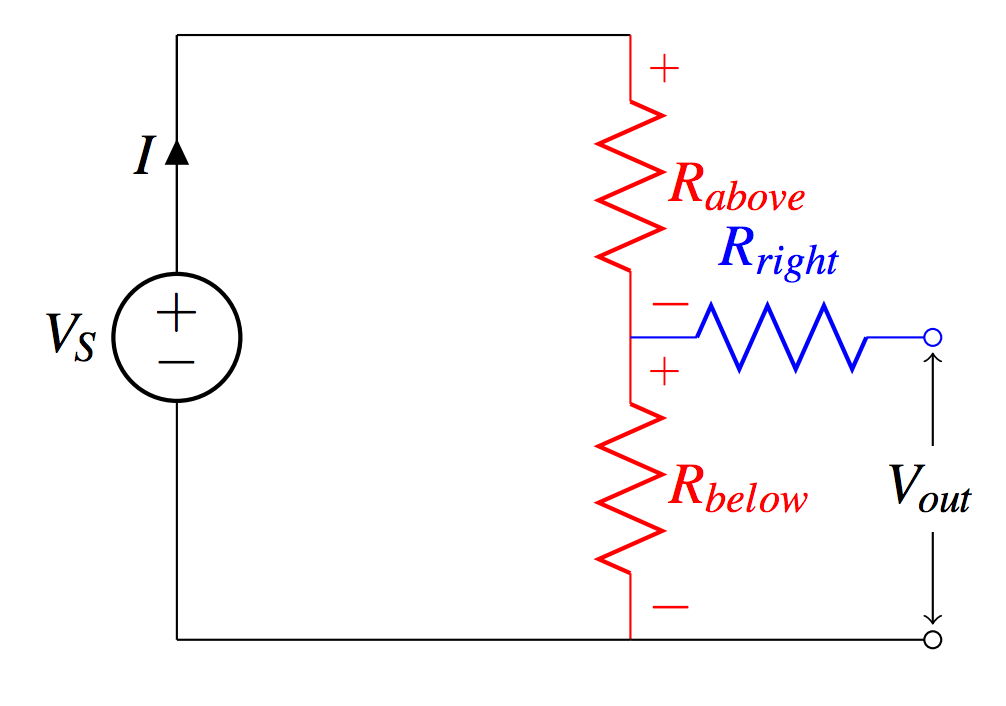
\includegraphics[scale=0.3]{vpos_simple.png}
     \end{align*}
     We obtain the proportion $h_{below}=\dfrac{V_{out}}{V_S}h$. \\
     Similarly, to measure horizontal position, we get this simplified circuit:
    \begin{align*}
        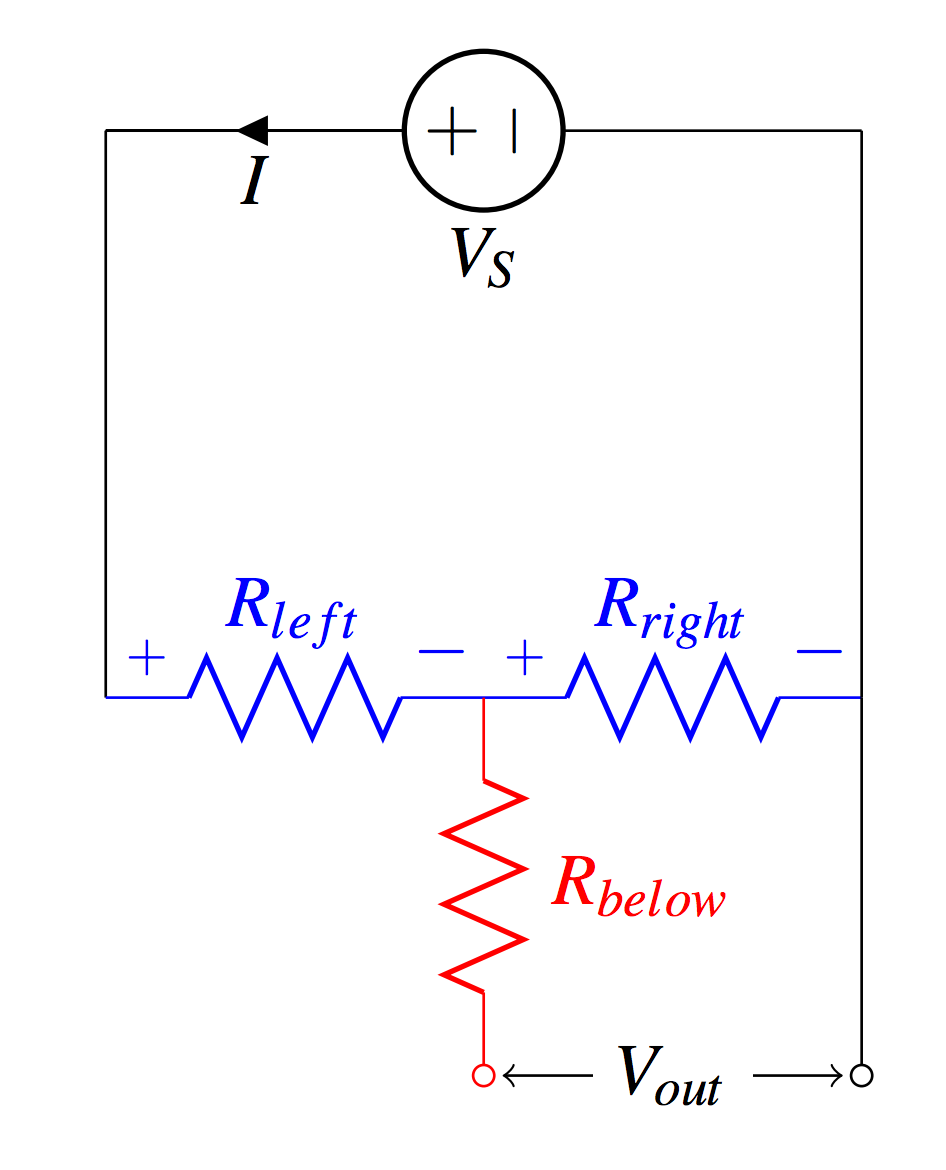
\includegraphics[scale=0.2]{hpos_simple.png}
     \end{align*}
     We obtain the proportion $w_{right}=\dfrac{V_{out}}{V_S}w$.
     
    \item 
    We can convert any circuit into a simplified circuit of two forms. \\ \textbf{Thevinin:}
    \begin{align*}
        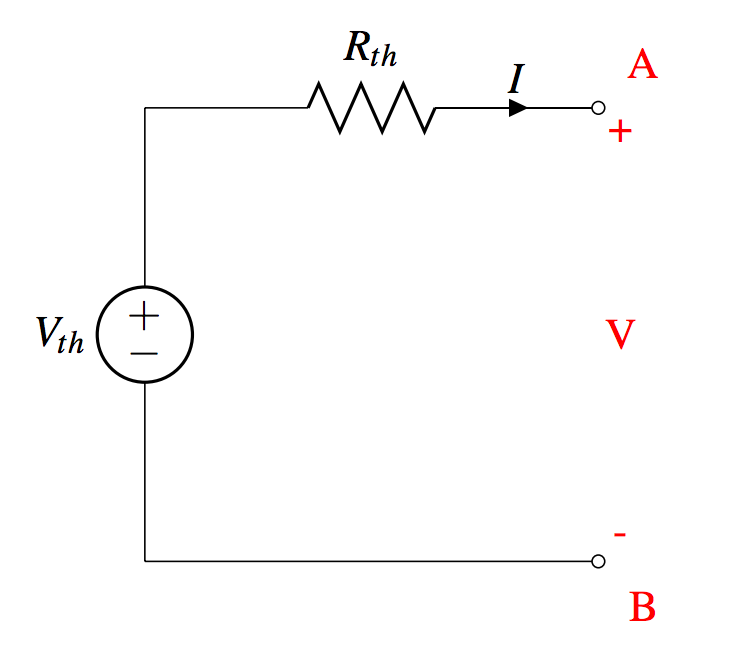
\includegraphics[scale=0.3]{thevinin.png}
     \end{align*}
     To find $V_{th}$, we leave the circuit open between A and B and solve for $V_{oc}$.To figure out $R_{th}$, we short A and B in the original circuit, find the current $I_{sc}$ going from A to B, and compute $R_{th} = \frac{V_{th}}{I_{sc}}$. For example, 
    \begin{align*}
        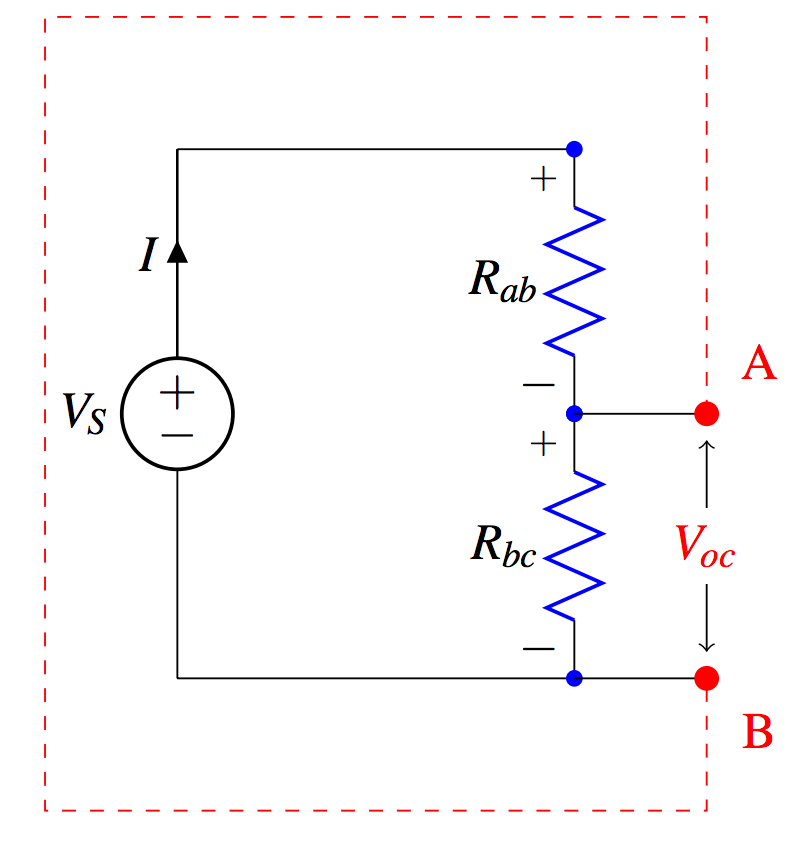
\includegraphics[scale=0.3]{ex1.png}
     \end{align*}
     here we see $V_{th}=V_{oc}=\frac{R_{bc}}{R_{ab}+R_{bc}}V_S$ and $R_{th} = \frac{V_{th}}{I_{sc}} = \frac{R_{ab}R_{bc}}{R_{ab}+R_{bc}}$. \\ \\
    \textbf{Norton:}
    \begin{align*}
    \vspace{-15ex}
        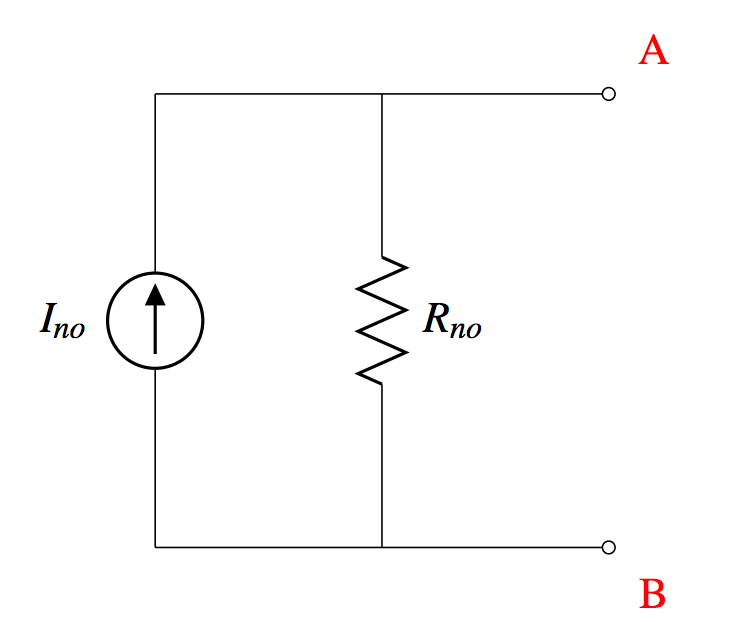
\includegraphics[scale=0.3]{norton.png}
     \end{align*}
     The procedure for finding $I_{no}$ and $R_{no}$ is exactly the same as that of finding $V_{th}$ and $R_{th}$. Using the sample example, the Norton equivalent circuit is 
    \begin{align*}
        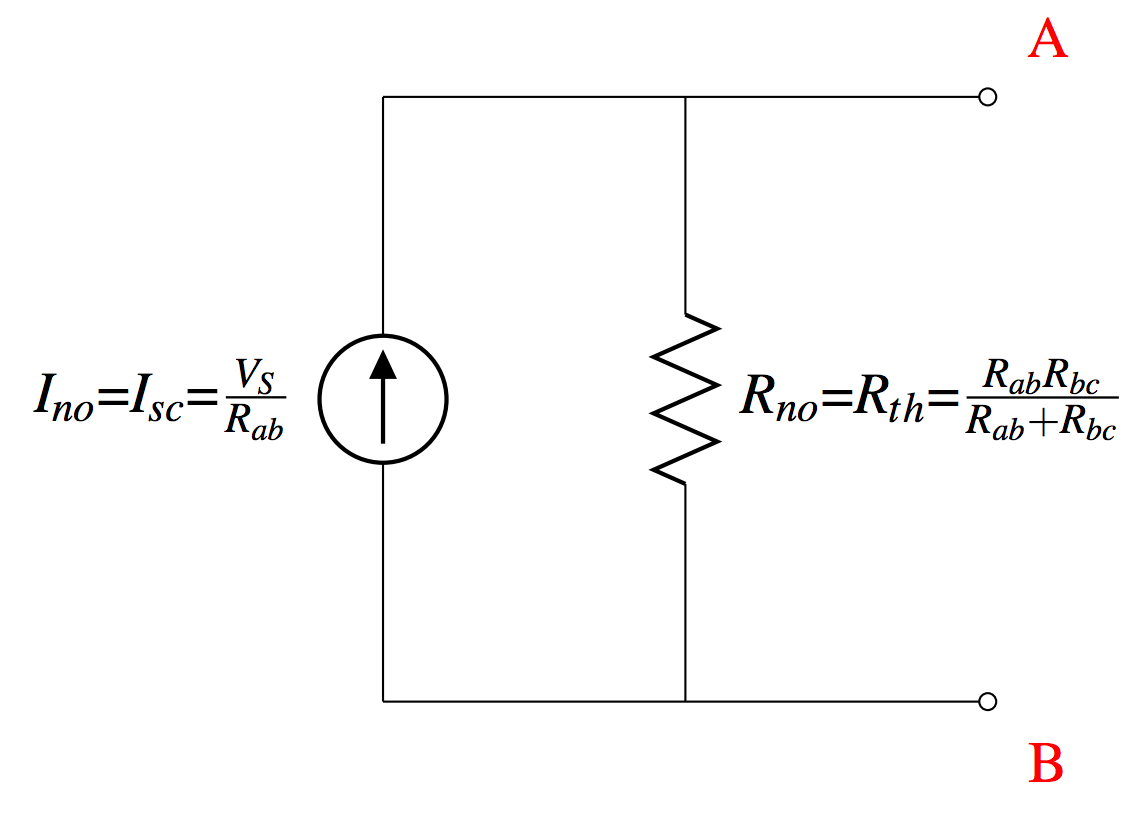
\includegraphics[scale=0.27]{ex2.png}
     \end{align*}

    \item \textbf{Superposition}: For circuits with multiple voltage or current sources: For each source $k$:
    \begin{itemize}
        \item 
            Voltage source: replace with a short circuit \\
            Current source: Replace with an open circuit

        \item Compute $V_{out,k}$ due to this source $k$
        \item Compute $V_{out}$ by summing the $V_{out,k}$s for all $k$.
    \end{itemize}
    
    \item \textbf{Capacitors}:\\
    \begin{enumerate}
        \item The energy stored across a capacitor after its been charged is $\frac{1}{2}CV^2$.
        \item For capacitors in series, we have: $$C_{eq}=\dfrac{1}{\frac{1}{C_1} + \frac{1}{C_2}} = \dfrac{C_1C_2}{C_1+C_2}$$
        \item For capacitors in parallel: $C_{eq} = C_1 + C_2$.
    \end{enumerate}
    
    \item \textbf{Capacitive Touchscreen Circuit:} \\
    The idea is to take a capacitor with variable capacitance (when touched vs not touched) and connect it to a fixed voltage $V$. There is $Q_{var}=C_{var}V$ charge on this capacitor. Then dump the charge on a fixed charge capacitor $C_{fixed}$. The voltage across this capacitor will be $V_{var}=\frac{Q_{var}}{Q_{fixed}}$. By measuing $V_{var}$, we can determine $C_{var}$. \\ The circuit:
    \begin{align*}
        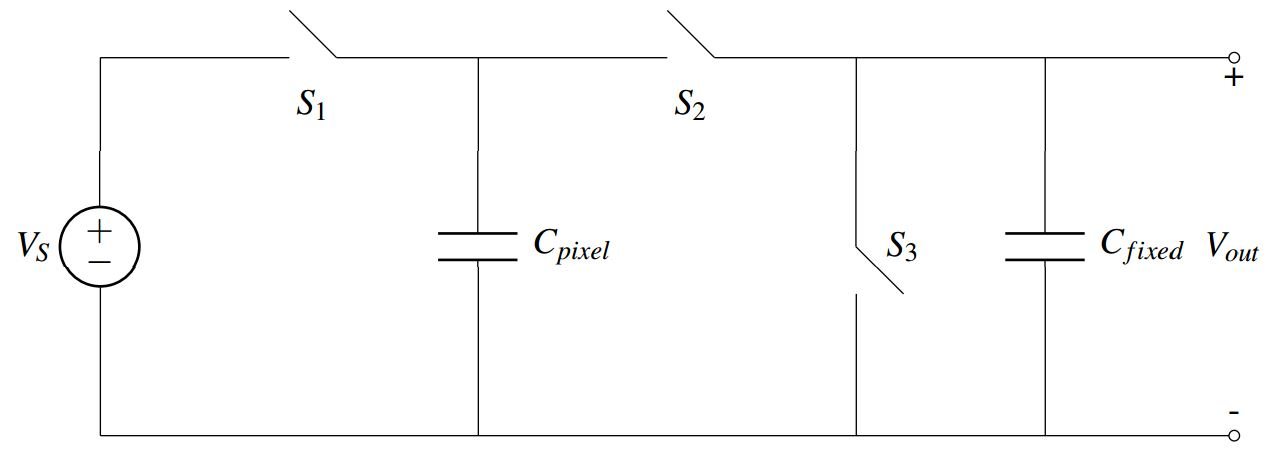
\includegraphics[scale=0.2]{ctc1.JPG}
     \end{align*}
    Phase 1: Charge $C_{pixel}$. The charge on $C_{pixel}$ is $Q_{pixel}=C_{pixel}V_S$. (And there is no charge on $Q_{fixed}$).
    \begin{align*}
        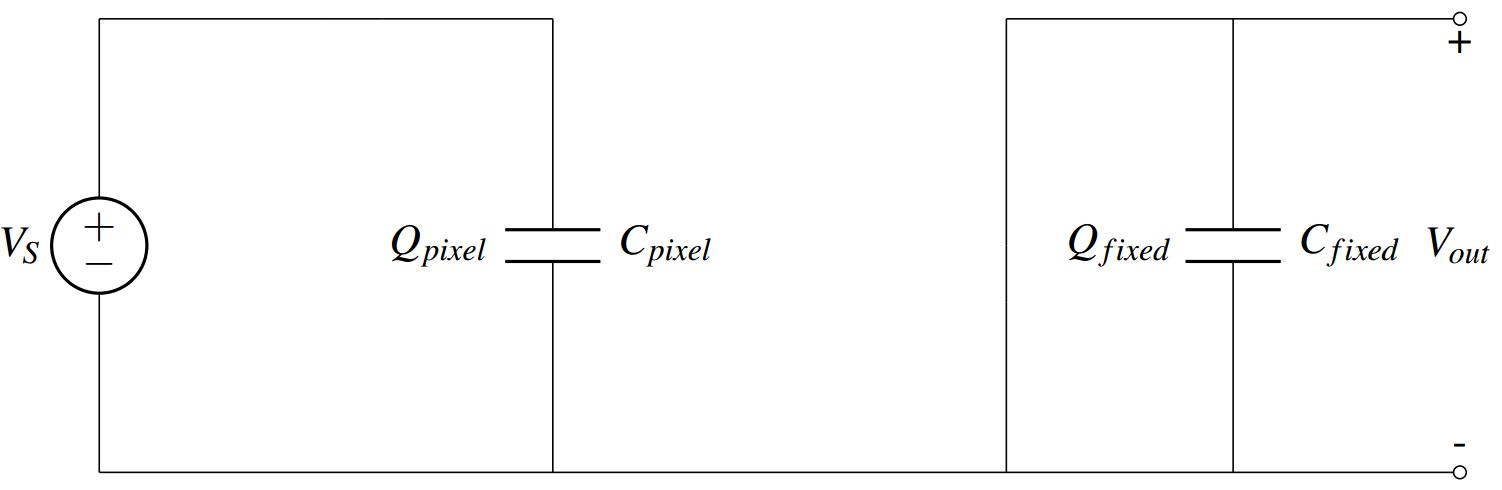
\includegraphics[scale=0.2]{ctc2.JPG}
     \end{align*}
    Phase 2 (Charge-sharing): 
    The total voltage is now the total charge available divided by the total capacitance. So we have: 
    \begin{equation*}
        V_{out}=\frac{C_{pixel}}{C_{pixel}+C_{fixed}}V_S
    \end{equation*}
    \begin{align*}
        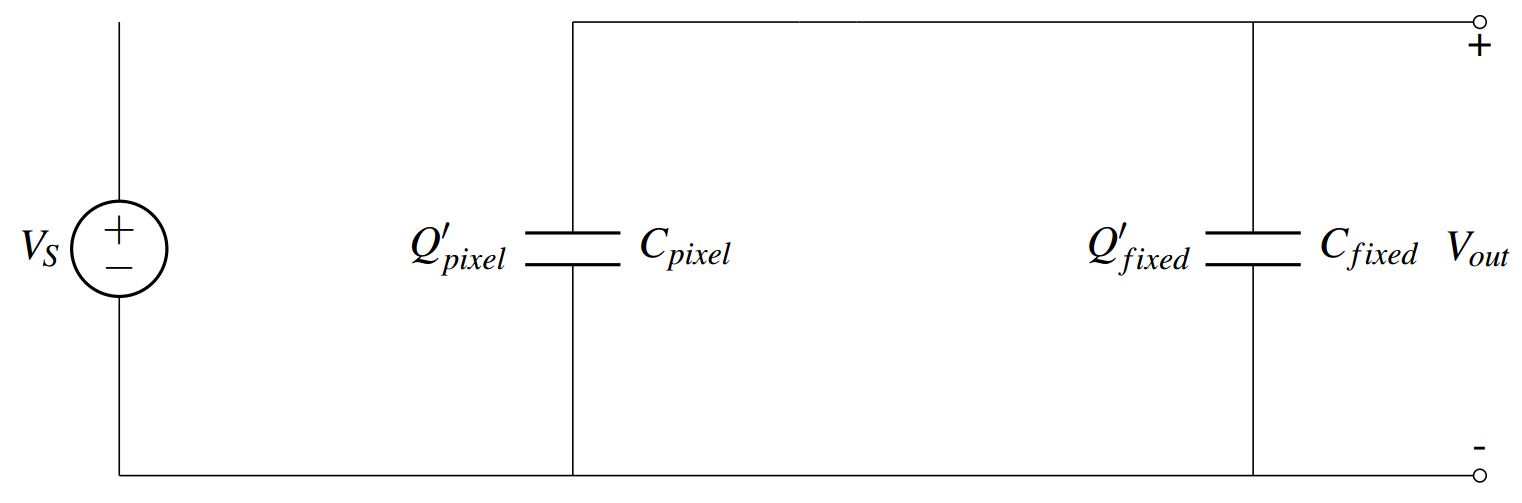
\includegraphics[scale=0.2]{ctc3.JPG}
     \end{align*}

    \item \textbf{Op Amps:}
    To measure $V_{out}$, there will be a finite resistance connected to the circuit. We introduce op-amps to help us prevent this resistance from causing the energy to be dissipated. 
    \begin{align*}
        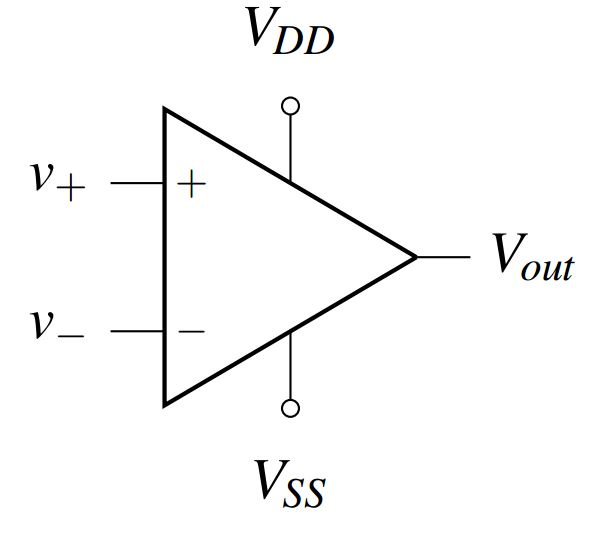
\includegraphics[scale=0.2]{OpAmp.JPG}
     \end{align*}
     This symbol represents the following equivalent circuits:
    \begin{align*}
        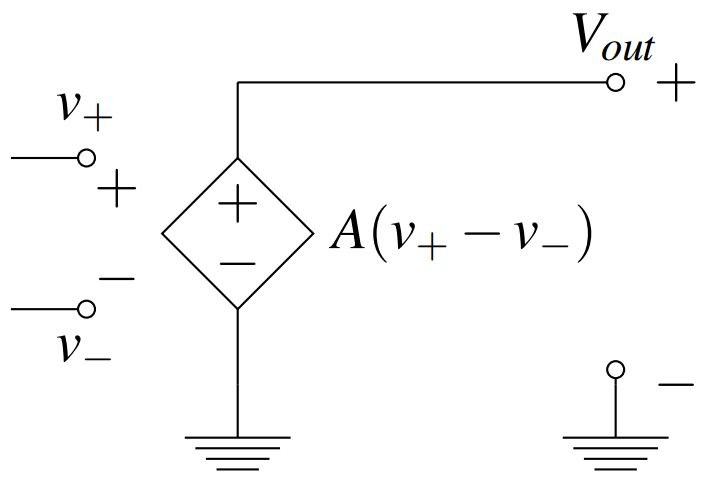
\includegraphics[scale=0.2]{OpAmp1.JPG}
     \end{align*}
    \begin{align*}
        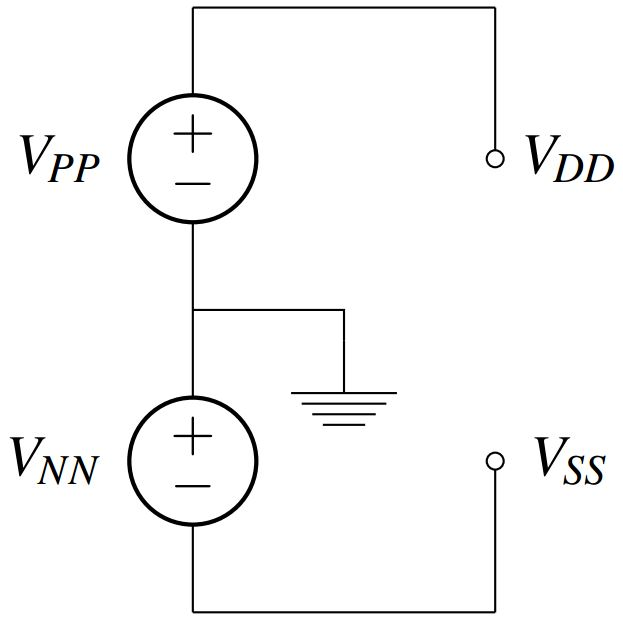
\includegraphics[scale=0.2]{OpAmp2.JPG}
     \end{align*}
    The voltage across the variable voltage source is $V_{out}=A(v_+-v_-)$ where $A$ is approaching infinity. However, $-V_{NN} \leq V_{out} \leq V_{PP}$. \\
    We attach an op-amp to the end of our circuit from above to obtain:
    \begin{align*}
        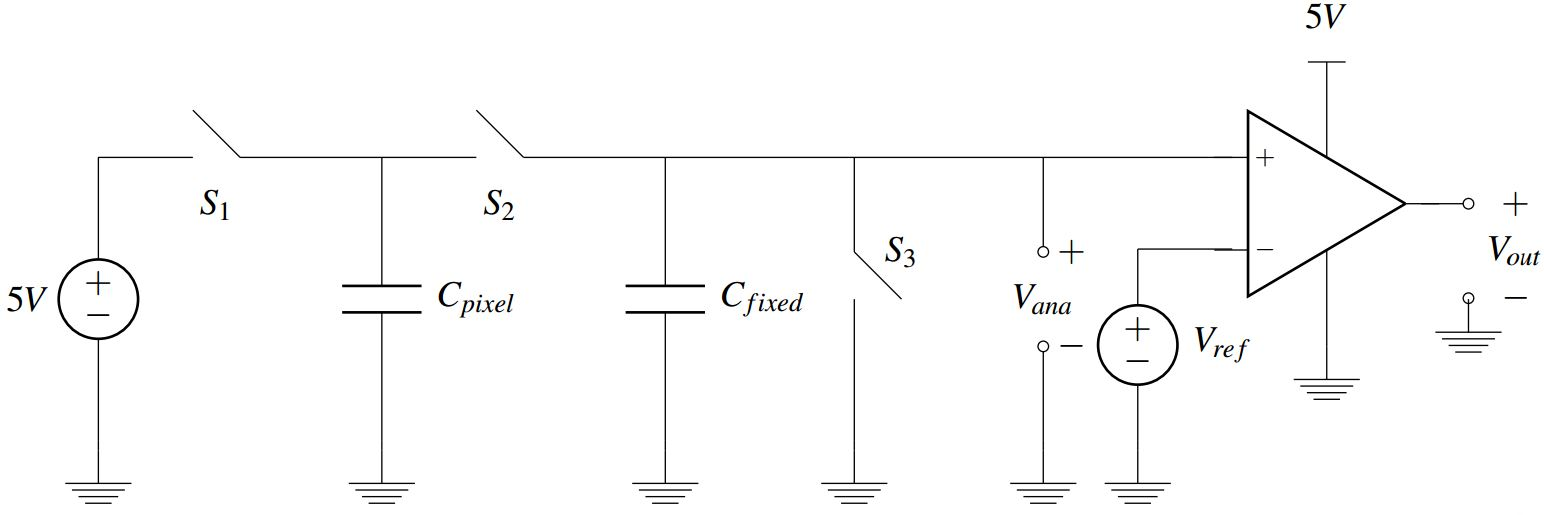
\includegraphics[scale=0.21]{OpAmp3.JPG}
     \end{align*}
     Note that the previous $V_{out}$ is now $V_{ana}$. Since
    \begin{equation*}
        V_{ana}=\frac{C_{pixel}}{C_{pixel}+C_{fixed}}V_S
    \end{equation*}
    We choose $C_{fixed}$ and $V_{ref}$ such that $V_{ana} > V_{ref}$ when there is a touch (so in this case $V_{out}=5V$) and $V_{ana} < V_{ref}$ when there is not a touch ($V_{out} =0V$).
    
    \item \textbf{2D Capacitive Touchscreen:}
    The arrangement (shaded is dielectric):
    \begin{align*}
        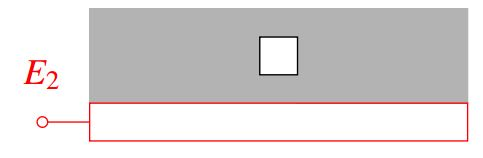
\includegraphics[scale=0.3]{ctcf1.JPG}
     \end{align*}
     The goal is to measure $C_{E_1-E_2}$. \\
    No touch:
    \begin{align*}
        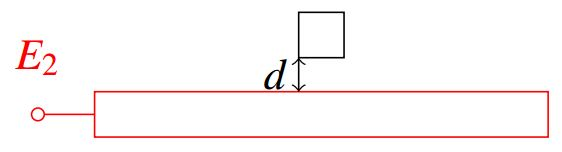
\includegraphics[scale=0.2]{ctcf2.JPG}
     \end{align*}
   $C_{E_1-E_2} = C_{no \hspace{1 mm} touch}$ 
    \begin{align*}
        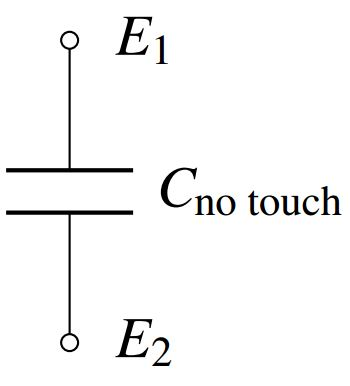
\includegraphics[scale=0.2]{ctcf3.JPG}
     \end{align*}
    With touch (blue line is finger touching dielectric):
    \begin{align*}
        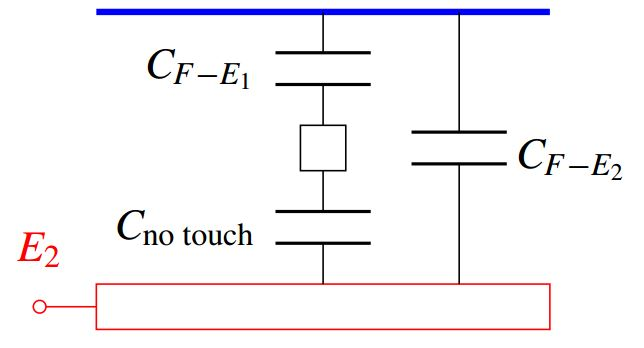
\includegraphics[scale=0.3]{ctcf4.JPG}
     \end{align*}
    In circuit form:
    \begin{align*}
        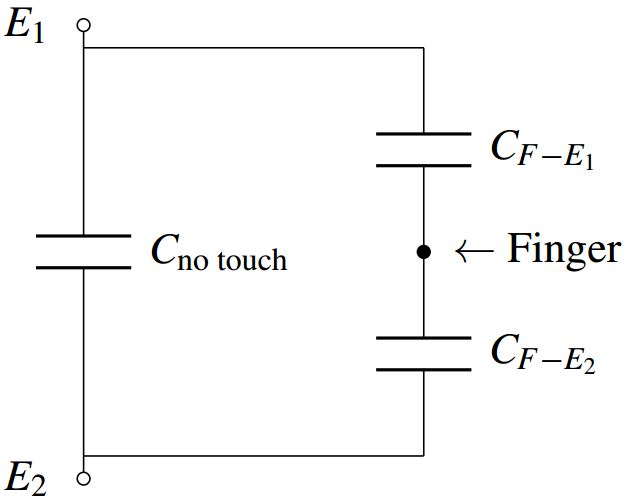
\includegraphics[scale=0.25]{ctcf5.JPG}
     \end{align*}
    $C_{E_1-E_2} = C_{no \hspace{1 mm} touch}+\frac{C_{F-E_1}C_{F-E_2}}{C_{F-E_1}+C_{F-E_2}}$ \\[6 pt]
    Use the same circuit from above to determine whether or not there was a touch.
    
     \item \textbf{Golden Rules:} 
     \begin{enumerate}
         \item $I^+=I^-=0$ No current flows across the +/- inputs of the op amp.
         \item $V^+=V^-$ In a circuit with negative feedback, the output of the op amp will adjust output so that the voltage difference between inputs is zero.
     \end{enumerate} 
    
    \item \textbf{Negative Feedback:} For negative feedback, the output is connected to the inverting input (- input). For positive feedback, the output is connected to the non-inverting input (+ input).
    
    \item \textbf{Basic Op-amp Circuits:} The goal of op-amp circuit analysis is to develop an expression for $V_{out}$ as a function of $V_{S}$ or $I_{S}$ and the resistances. Note that in all these cases, the voltage ratio depends only on the ratio of resistances, so errors cancel out. \\
    The general process is as follows: Choose arbitrary current directions and label with arrows. Use $V_+=V_-$ to gain some insight (one terminal is usually connected to ground or a voltage source). Apply KCL at the $V_-$ node. Then express currents in terms of voltage across it (use direction of arrow) and resistances. Solve from here. \\
    \textbf{Inverting amplifier:}
    \begin{align*}
        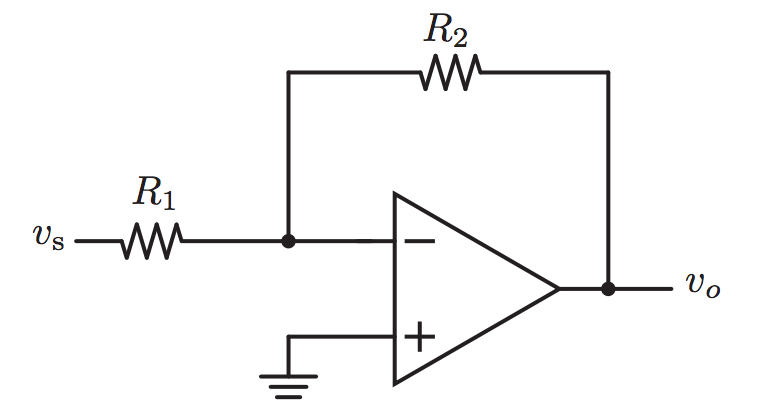
\includegraphics[scale=0.2]{inverting.png}
     \end{align*}
     We see that $V_-=V_+=0$. Use KCL at the junction and convert to voltage/resistance by : \\
     \begin{align*}
        I_{1} + I_2 = 0 \\
        \frac{V_{S}-V_-}{R_{1}} + \frac{V_o-V_-}{R_2} = 0 \\
        - \frac{V_{S}}{R_{1}} =  \frac{V_o}{R_2}
     \end{align*}
     Hence
     \begin{align*}
         V_{o}=- \frac{R_2}{R_{1}}V_{S}
     \end{align*}
     \textbf{Noninverting Amplifier:}
    \begin{align*}
        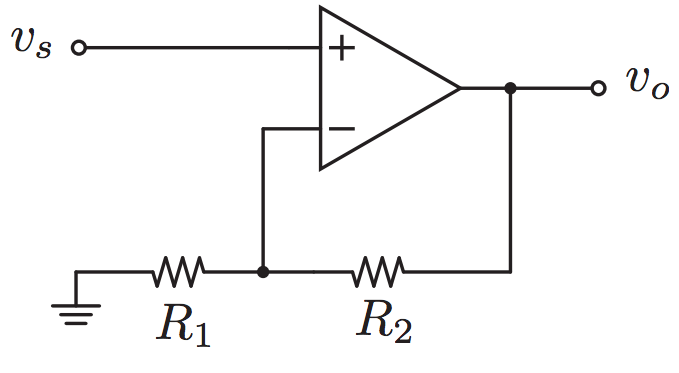
\includegraphics[scale=0.2]{noninverting.png}
     \end{align*}
     We see that $V_-=V_+=V_S$. Use KCL at the junction and convert to voltage/resistance by : \\
     \begin{align*}
        I_1+I_2=0 \\
        \frac{0-V_-}{R_1} + \frac{V_o-V_-}{R_2} = 0 \\
        \frac{V_S}{R_1} = \frac{V_{o}-V_S}{R_2} \\
     \end{align*}
     Move terms around to get:
     \begin{align*}
         V_{o}=V_{S}(1+\frac{R_2}{R_{1}})
     \end{align*}
     
     
\item \textbf{Inner Products} \\
    The dot product of vectors $\vec{u}$ and $\vec{v}$ $\in$ $\mathbb{R}^n$ is defined as:
    \begin{equation*}
       \langle \vec{u} , \vec{v} \rangle = \vec{u}^T\vec{v} = \begin{bmatrix} u_1 & \hdots & u_n \end{bmatrix}
        \begin{bmatrix} v_1 \\ \vdots \\ v_n \end{bmatrix}
       = u_1v_1+\ldots u_nv_n
    \end{equation*}
    Properties:
    \begin{align*}
        \langle \vec{u} , \vec{v} \rangle  = \langle \vec{v} , \vec{u} \rangle \\
        \langle c\vec{u} , \vec{v} \rangle = c\langle \vec{u} , \vec{v} \rangle \\
        \langle \vec{u} +\vec{x}, \vec{v} \rangle = \langle \vec{u} , \vec{v} \rangle + \langle \vec{x} , \vec{v} \rangle
    \end{align*}
    The Euclidean norm (length) of a vector is defined as:
    \begin{equation*}
        \norm{\norm{\vec{u}}}=\sqrt{\langle \vec{u}, \vec{u} \rangle}
    \end{equation*}
    For vector lengths:
    \begin{equation*}
        \langle \vec{u}, \vec{v} \rangle=\norm{\norm{\vec{u}}}\hspace{.5mm}\norm{\norm{\vec{v}}}\cos{\theta}
    \end{equation*}
    Cauchy-Schwartz Inequality:
    \begin{align*}
        \norm{\langle\vec{x},\vec{y}\rangle} \leq  \norm{\norm{\vec{x}}} \cdot \norm{\norm{\vec{y}}}
    \end{align*}
    The projection of a vector $\vec{y}$ onto another vector $\vec{x}$ is given by:
    \begin{align*}
        \Est{y} = \frac{\langle \vec{y} , \vec{x} \rangle}{\langle \vec{x} , \vec{x} \rangle}\vec{x}
    \end{align*}
    Similarly, the projection of a vector $\vec{y}$ onto a subspace $W$ is given by
    \begin{align*}
        \Est{y} = \frac{\langle \vec{y} , \vec{u_1} \rangle}{\langle \vec{u_1} , \vec{u_1} \rangle}\vec{u_1}
        + \hdots + \frac{\langle \vec{y} , \vec{u_n} \rangle}{\langle \vec{u_n} , \vec{u_1} \rangle}\vec{u_n}
    \end{align*}
    where $\left\{\vec{u_1}, \hdots, \vec{u_n}\right\}$ form an orthogonal basis for $W$. 
    \item \textbf{Correlations} \\ We use inner products as a similarity measure between vectors in the context of
    searching for a time-shift of a beacon signal. We cross-correlate a signal $\vec{s_1}$ and signal $\vec{s_2}$ by first constructing the circulant matrix $C_{\vec{s_1}}$ of $\vec{s_1}$ (an $N$ x $N$ matrix whose $i^{th}$ column is the $i^{th}$ rotation of $\vec{s_1}$; this matrix should be approximatelty orthogonal). Then the cross-correlation of $\vec{s_2}$ with all shifts of $\vec{s_1}$ is $C_{\vec{s_1}}^T\vec{s_2}$. The index of the maximum of the plot of this vector represents the time-delay of the signal. Autocorrelation is cross-correlating a vector with itself.
    
    \item \textbf{Triangulation} \\ After finding the time-delays of signals, we can find the distances to each beacon based on knowing the speed of the wave. Assuming we know the locations of the beacons, we can now find our position. 
    \begin{align*}
        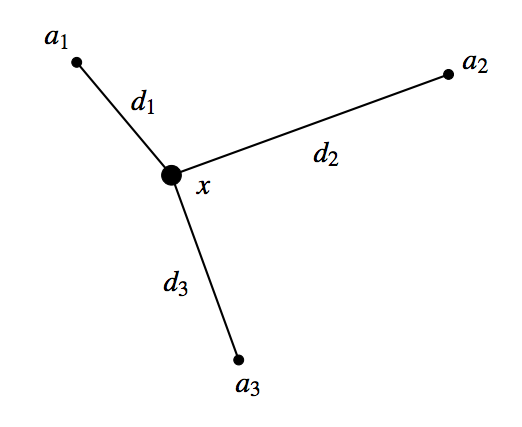
\includegraphics[scale=0.25]{loc.png}
    \end{align*}
    Using some tricks to make the terms linear, we can solve for $\vec{x}$ with
    \begin{align*}
        \begin{bmatrix} 
        2 \left( \vec{a_1}-\vec{a_2} \right)^T \\
        2 \left( \vec{a_1}-\vec{a_3} \right)^T 
        \end{bmatrix}
        \vec{x} = 
        \begin{bmatrix}
        \norm{\norm{\vec{a_1}}}^2-\norm{\norm{\vec{a_2}}}^2-d_1^2+d_2^2 \\
        \norm{\norm{\vec{a_1}}}^2-\norm{\norm{\vec{a_3}}}^2-d_1^2+d_3^2 
        \end{bmatrix}
    \end{align*}
    
    \item \textbf{Least Squares} \\ The set of least squares solutions to $A\vec{x}=\vec{b}$ is the set of solutions to $A^TA\vec{x}=A^T\vec{b}$. $A^TA$ must be invertible, which occurs iff $A$ has linearly independent columns. \\ A common application of least squares involves curve fitting. Suppose we have points $\left( x_1, y_1 \right), \hdots, \left( x_n, y_n \right)$ and we would like to put them in the form $y=ax+b$ (a line). In matrix form:
    \begin{align*}
        \begin{bmatrix}
        x_1 & 1 \\
        x_2 & 1 \\
        \vdots & \vdots \\
        x_n & 1
        \end{bmatrix}
        \begin{bmatrix}
        a \\
        b
        \end{bmatrix} = 
        \begin{bmatrix}
        y_1 \\ y_2 \\ \vdots \\ y_n
        \end{bmatrix}
    \end{align*}
    Apply least squares to solve for $a,b$. The mean squared error is given by 
    \begin{align*}
        \norm{\norm{\vec{b} - A\begin{bmatrix} a \\ b \end{bmatrix}}}^2
    \end{align*}
    Alternatively, suppose we would like to fit them to $ax^2+bxy+cy^2+dx+ey=1$ (an ellipse). We set up the following matrix:
    \begin{align*}
        \begin{bmatrix} 
        x^2_1 & x_1y_1 & y^2_1 & x_1 & y_1 \\
        \vdots & \vdots & \vdots & \vdots & \vdots \\
        x^2_n & x_ny_n & y^2_n & x_n & y_n
        \end{bmatrix}
        \begin{bmatrix} 
        a \\ b \\ c \\ d \\ e
        \end{bmatrix} =
        \begin{bmatrix} 1 \\ \vdots \\ 1 \end{bmatrix}
    \end{align*}
    
    \item \textbf{Gram-Schmidt Process} \\ Given a basis $W = \left\{\vec{x_1}, \hdots, \vec{x_n} \right\}$, we can construct an orthogonal basis. Let
    \begin{align*}
        \vec{v_1}=\vec{x_1} \\
        \vec{v_2}=\vec{x_2} - \left( \frac{\langle\vec{x_2}, \vec{v_1}\rangle}{\langle \vec{v_1}, \vec{v_1} \rangle}\vec{v_1} \right) \\
        \vec{v_3}=\vec{x_3} - \left( \frac{\langle\vec{x_3}, \vec{v_1}\rangle}{\langle \vec{v_1}, \vec{v_1} \rangle}\vec{v_1} + \frac{\langle\vec{x_3}, \vec{v_2}\rangle}{\langle \vec{v_2}, \vec{v_2} \rangle}\vec{v_2} \right) \\
        \vdots
    \end{align*}
    
    \item \textbf{Orthogonal Matching Pursuit} \\ The message signal is a vector of real numbers and the signature codes (which are known) are streams of $\pm$ 1, which have a high auto-correlation and low cross-correlation with other codes. The signature codes are multiplied with the appropriate message signal to get the transmission signal. The signal received at the tower is a (assumed sparse) linear combination of shifts of signals from all transmitting users scaled by an attenuation factor:
    $$\vec{y} = \sum_{i=1}^{d} \alpha_i \vec{S}_i$$
    where $d$ is the number of unique signatures, $\vec{S_i}$ is the $i^{th}$ column vector of the signature matrix $S$, and $\alpha_i$ is the message. The process (assuming no shifts):
    \begin{enumerate}
        \item Initialize the residual vector $\vec{r}=\vec{y}$. Let $A$ be the initially empty matrix made of found signatures.
        \item Find vector $\vec{S_i}$ (not chosen before) with highest correlation with $\vec{r}$. $k=\argmax_i{\langle \vec{S_i}, \vec{r} \rangle}$. Append $\vec{S_k}$ to $A$.
        \item Use least squares to project $\vec{r}$ onto subspace spanned by previously found $\vec{S_i}$'s: $\vec{\Est{r}}=A(A^TA)^{-1}A^T\vec{r}$.
        \item Reset $\vec{r}=\vec{r}-\Est{\vec{r}}$. Repeat the above $m$ times, the sparsity level of the signal.
        \item Solve for the messages $\alpha_i$ by computing $(A^TA)^{-1}A^T\vec{y}$.
    \end{enumerate}
    The procedure is made much faster by orthonormalizing the found vector using Gram-Schmidt before appending to $A$. After this, step (c) becomes $\vec{\Est{r}}=\langle \vec{v_1} , \vec{r} \rangle \vec{v_1} + \hdots + \langle \vec{v_n} , \vec{r} \rangle \vec{v_n}$ where $\vec{v_n}$ are the columns of $A$.
    
    \item \textbf{Pagerank} Representing websites as nodes and links to other sites as directed edges, the Internet can be modeled as a pump system with a corresponding transition matrix. If we think of the initial viewers per page $\vec{x}[0]$ as fractions that sum to 1, then the fraction of viewers at time $k$ is $T^k\vec{x}[0]$, where $T$ is the transition matrix. \\
    Assuming $\vec{x}[k]$ converges to some stable fractions, that is, there exists $\vec{x}_{SS}$ such that $P\vec{x}_{SS}=\vec{x}_{SS}$ where $P$ is some power of $T$, we can find this steady-state vector by finding a corresponding eigenvector for $\lambda = 1$. If the number of viewers is preserved, we can easily find the appropriate scalar for the eigenvector to get $\vec{x}_{SS}$.
    
    \item \textbf{Determinants} The determinant of a 2 x 2 matrix $A$ is $det \left( \begin{bmatrix} a & b \\ c & d \end{bmatrix} \right)=ad-bc$. For an upper or lower triangular matrix, the determinant is the product of the diagonal entries. The determinant is the product of eigenvalues of a matrix.
    
    \item \textbf{Trace} The trace of a matrix, $tr(A)$, is  the sum of the entries on the diagonal. It is equal to the sum of the eigenvalues of a matrix.
    
    \item \textbf{Eigenvalues/Eigenvectors} We compute eigenvalues by solving for the roots of $det( A-\lambda I)=0$. The eigenvectors associated with an eigenvalue $\lambda$ is given by $Nul(A - \lambda I)$.
    
    \item \textbf{Diagonalization} A diagonalizable matrix $A$ is one that has $n$ linearly independent eigenvectors and can be written as 
    $$A=PDP^{-1}= $$
    \begin{align*}
        \begin{bmatrix} 
        | & & | \\
        \vec{v_1} & \hdots & \vec{v_n} \\
        | & & |
        \end{bmatrix}
        \begin{bmatrix}
        \lambda_1^N & \hdots & 0 \\
        \vdots & \ddots & \vdots \\
        0 & \hdots & \lambda_n^N
        \end{bmatrix}
        \begin{bmatrix} 
        | & & | \\
        \vec{v_1} & \hdots & \vec{v_n} \\
        | & & |
        \end{bmatrix}^{-1}
    \end{align*}
    
    \item \textbf{Change of basis}     
    For bases
    \begin{align*}
        A= \left\{ \begin{bmatrix} 1 \\ 0 \end{bmatrix}, \begin{bmatrix} 1 \\ 1 \end{bmatrix} \right\}, 
        B= \left\{ \begin{bmatrix} 1 \\ 1 \end{bmatrix}, \begin{bmatrix} 1 \\ 2 \end{bmatrix} \right\}
    \end{align*}
    The matrix $T$ such that $\vec{x}_B=T\vec{x}_A$ is 
    \begin{align*}
        T=\begin{bmatrix}
        \begin{bmatrix} 1 \\ 0 \end{bmatrix}_B & \begin{bmatrix} 1 \\ 1 \end{bmatrix}_B 
        \end{bmatrix} =
        \begin{bmatrix}
        2 & 1 \\ -1 & 0 
        \end{bmatrix}
    \end{align*}
    
    \item \textbf{Rotation matrix} The matrix that rotates a given vector by a counterclockwise angle $\theta$: 
    \begin{equation*}
        \begin{bmatrix} 
        \cos{\theta} & -\sin{\theta} \\
        \sin{\theta} & \cos{\theta}
        \end{bmatrix}
    \end{equation*}
\end{enumerate}

\end{multicols}
\end{document}
